% Fig (method, panel c) - Evaluation protocol for vortex-jepa manuscript.
%
% Shows that the same predictor architecture and probe family map every encoder family
% (JEPA, AE, POD) to the same observables, in two modes:
%   representation closure: probe on the simulation-encoded latent z_t
%   forecast closure:       probe on the rolled-out latent zhat_{t+H}
%
% Standalone-compilable: pdflatex fig_eval_protocol.tex

\documentclass[border=10pt,tikz]{standalone}
\usepackage{tikz}
\usepackage{amsmath,amssymb}
\usetikzlibrary{positioning,arrows.meta,fit,shapes.geometric,calc,backgrounds}

\begin{document}

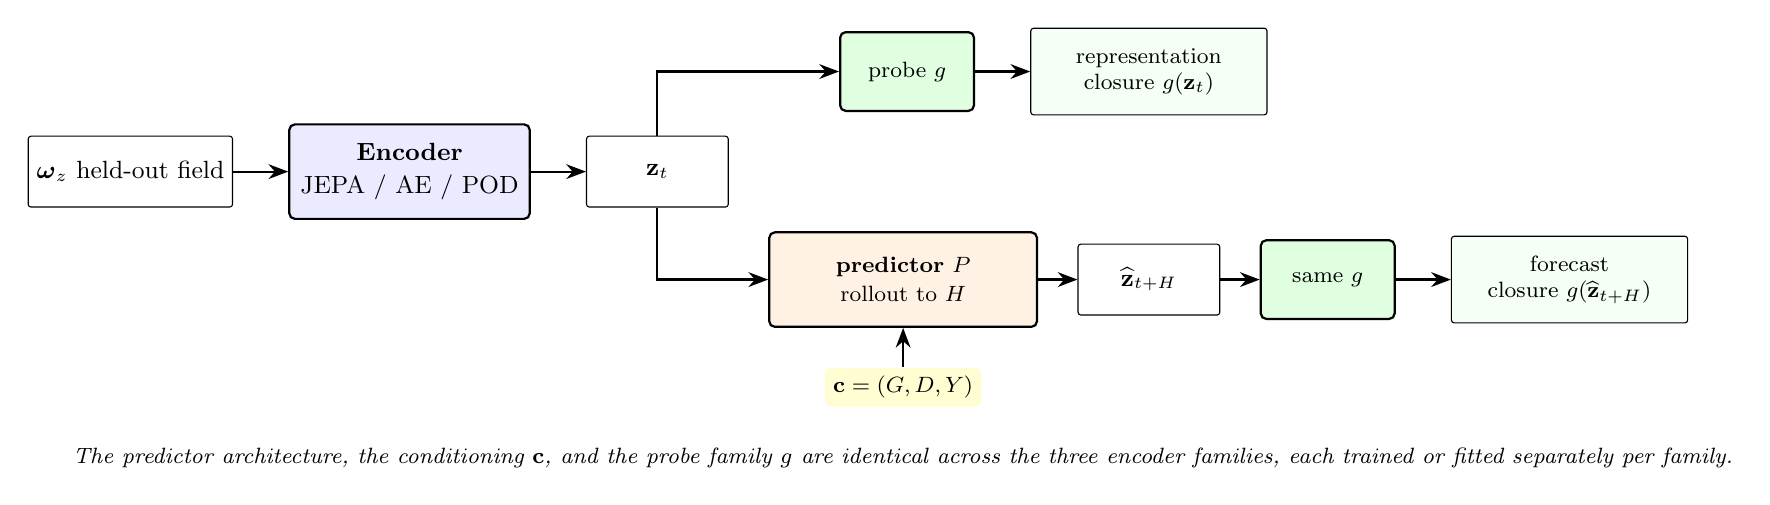
\begin{tikzpicture}[
    font=\small,
    box/.style={draw, rounded corners=2pt, align=center, inner sep=4pt, thick},
    encoder/.style={box, fill=blue!8,  minimum width=26mm, minimum height=12mm},
    predictor/.style={box, fill=orange!10, minimum width=34mm, minimum height=12mm,
                      font=\footnotesize},
    probe/.style={box, fill=green!12, minimum width=17mm, minimum height=10mm,
                  font=\footnotesize},
    state/.style={draw, rectangle, rounded corners=1pt, fill=white,
                  minimum height=9mm, minimum width=18mm, inner sep=3pt},
    obs/.style={draw, rectangle, rounded corners=1pt, fill=green!4,
                minimum height=11mm, minimum width=30mm, inner sep=3pt,
                font=\footnotesize, align=center},
    arr/.style={-{Stealth[length=2.5mm]}, thick}
  ]

  % ---- shared front end ----
  \node[state] (field) {$\boldsymbol{\omega}_z$ \\[1pt] held-out field};
  \node[encoder, right=7mm of field] (enc)
    {\textbf{Encoder} \\[1pt] JEPA / AE / POD};
  \node[state, right=7mm of enc] (zt) {$\mathbf{z}_t$};
  \draw[arr] (field) -- (enc);
  \draw[arr] (enc) -- (zt);

  % ---- top branch: representation closure ----
  \node[probe, above right=3mm and 14mm of zt] (probeR) {probe $g$};
  \node[obs, right=7mm of probeR] (obsR)
    {representation \\ closure $g(\mathbf{z}_t)$};
  \draw[arr] (zt.north) |- (probeR.west);
  \draw[arr] (probeR) -- (obsR);

  % ---- bottom branch: forecast closure ----
  \node[predictor, below right=3mm and 5mm of zt] (pred)
    {\textbf{predictor} $P$ \\[1pt] rollout to $H$};
  \node[state, right=5mm of pred] (zhat) {$\widehat{\mathbf{z}}_{t+H}$};
  \node[probe, right=5mm of zhat] (probeF) {same $g$};
  \node[obs, right=7mm of probeF] (obsF)
    {forecast \\ closure $g(\widehat{\mathbf{z}}_{t+H})$};
  \draw[arr] (zt.south) |- (pred.west);
  \draw[arr] (pred) -- (zhat);
  \draw[arr] (zhat) -- (probeF);
  \draw[arr] (probeF) -- (obsF);

  % ---- conditioning into the predictor ----
  \node[align=center, font=\footnotesize, fill=yellow!18, rounded corners=2pt,
        inner sep=3pt, below=5mm of pred] (cond)
    {$\mathbf{c}=(G,D,Y)$};
  \draw[arr] (cond.north) -- (pred.south);

  % ---- annotation ----
  \node[align=center, font=\footnotesize\itshape, below=4mm of cond]
    {The predictor architecture, the conditioning $\mathbf{c}$, and the probe family
     $g$ are identical across the three encoder families, each trained or fitted
     separately per family.};

\end{tikzpicture}

\end{document}
